% 20200719
\documentclass[../thesis.tex]{subfiles} %% use packages & commands as this main file
\begin{document}
Biomass densities were stable within days in destructive systems.  \Phy\ biomass densities in both systems dropped during system development (Fig.\ref{f:destCarbon}B).  \Bac\ density had a increase and set back a little to the stable level (Fig.\ref{f:destCarbon}C).  Organic carbon in both systems behaved differently (Fig.\ref{f:destCarbon}A).  It accumulated linearly in \PoN\ but dropped to stability level in \PBN.  Daily yield was significantly different (Fig.\ref{f:ydByHarv}A; p $\ll$ 0.01) between systems or across time except \PoN\ system after the first few days of system development (Fig.\ref{f:ydDaily}A \& \ref{f:ydByHarv}A; p$>$0.1 for \PoN\ day 5 \& 50).  Yield level plateau at long runtime for \phy-only systems but it peaked early in \PBN\ systems (Fig.\ref{f:ydDaily}).  Yet \phy-only systems always had a higher yield distribution than \pbs s with less \phy\ biomass (Fig.\ref{f:destCarbon}B).

Feasible systems in continuous harvest modes had positive yields.  Favourable systems in destructive harvest modes had yields higher than initial values.  \Phy-only systems were all feasible but not all \pbs s (Table \ref{t:feasDist}).  Destructive harvest for \pbs s (\PBN) were mostly feasible with an almost-zero expected yield.  Continuous harvest for \pbs s (\PBH) had most of its systems unfeasible but expected yields were higher than other systems among feasible scenarios.  Most system pairs showed significance in median difference (\PoH\ vs \PoN: p=0.36; other pairs: p$\ll$0.01).  \Bac l invasion into \PoN\ systems would largely reduce its expected yield (Fig.\ref{f:bacEffect}).  With the right combination of \phy\ and \bac, \pbs s could also have yield comparable with \phy-only systems.

\begin{table}[H]
    \centering
    \caption[Yield distribution summary]{Feasible yield distribution summary of the harvest interval/rate with maximum yield}
    \begin{tabular}{ccrrcccc}\hline
        System & max & scenarios & \% & lower quartile & median & upper quartile & max \\
        & $x$ or $T$ & (N=5500) && \dxdt & \dxdt & \dxdt & \dxdt \\\hline
        \PBH & 2101 \dayU & 19 & 0.3 & 12.4 & 25.2 & 47.8 & 285 \\
        \PBN & 90 days & 5346 & 97.2 & -0.012 & 0.019 & 0.141 & 243 \\
        \PoH & 19501 \dayU & 5500 & 100.0 & 0.039 & 0.371 & 1.853 & 346 \\
        \PoN & 19900 days & 5500 & 100.0 & 0.045 & 0.379 & 1.851 & 346 \\
    \hline\end{tabular}
    \label{t:feasDist}
\end{table}

Most \phy\ biology had significant (p$\ll$0.01 for Wilcox test across the ends of parameter ranges) unidirectional ($\ePR$, $\eP$, $\gP$: positive; $\aP$: negative) effect on log yield distributions (Fig.\ref{f:bacEffect}).  \Bac\ biology had no observable distribution influences (Fig.\ref{f:bacEffect2}).  Harvest modes determined feasibility of \pbs s (Fig.\ref{f:harvPB}) but had no effect on \phy-only systems (Fig.\ref{f:harvPo}).  In short, yield distribution maximized when \phy\ had high carbon-to-biomass ratio (high $\ePR$ and $\eP$), high growth rate (high $\gP$) and low intraspecific interference (low $\aP$).

\begin{figure}[H]
    \centering
    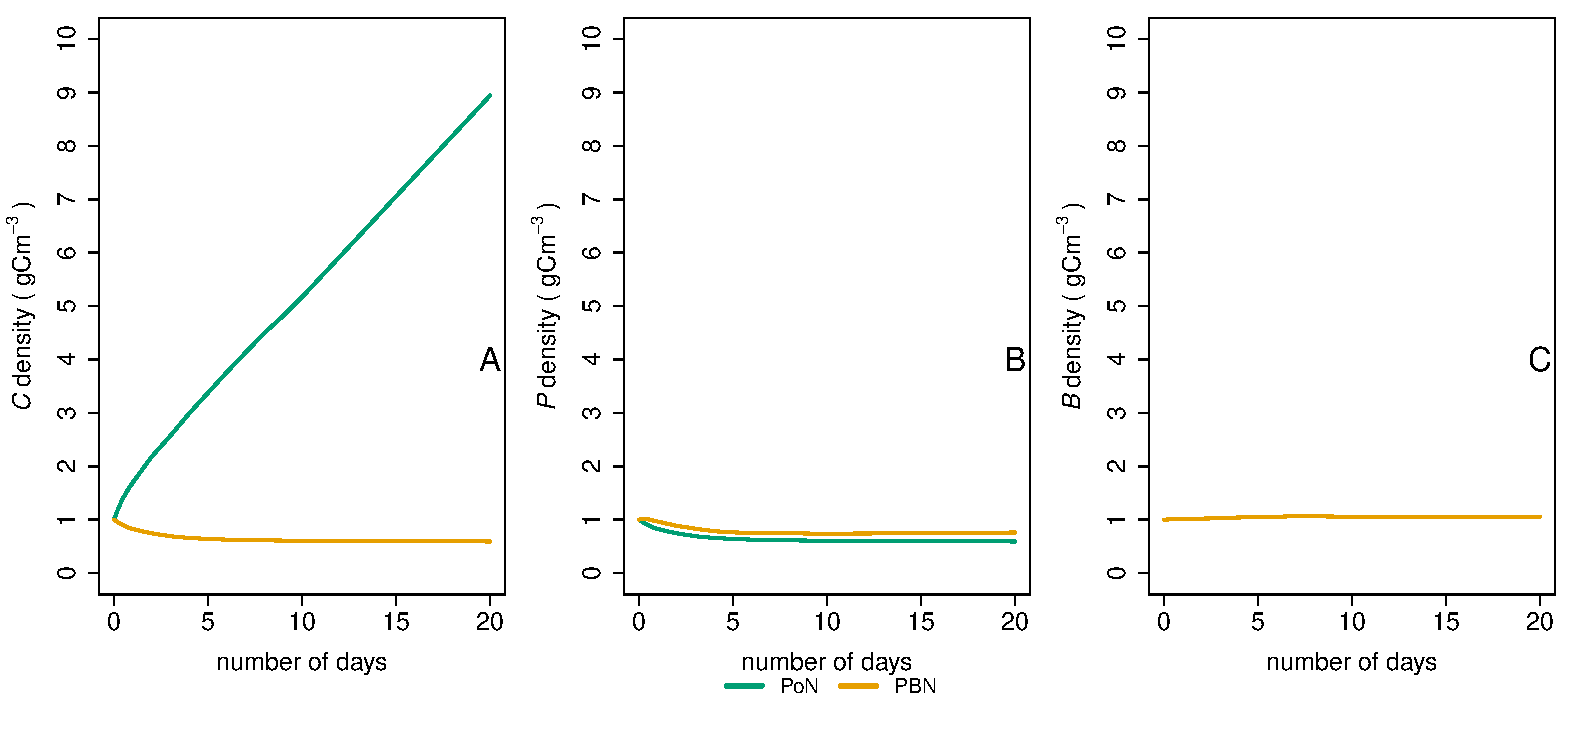
\includegraphics[width=\linewidth]{result/Sample.pdf}
    \caption[Median carbon content in destructive systems]{Median carbon content in destructive systems.  \textbf{(A)}, \textbf{(B)} and \textbf{(C)} showed carbon densities in respective carbon pools since establishment.  Initial carbon densities for \PoN\ were [1,1,0]\den\ ($C$, $P$, $B$) and that for \PBN\ were [1,1,1]\den\ modeled from Eq.\ref{eq:PBH}.  Note that \PoN\ carbon accumulation was linear after establishment.}
    \label{f:destCarbon}
\end{figure}

\begin{figure}[H]
    \centering
    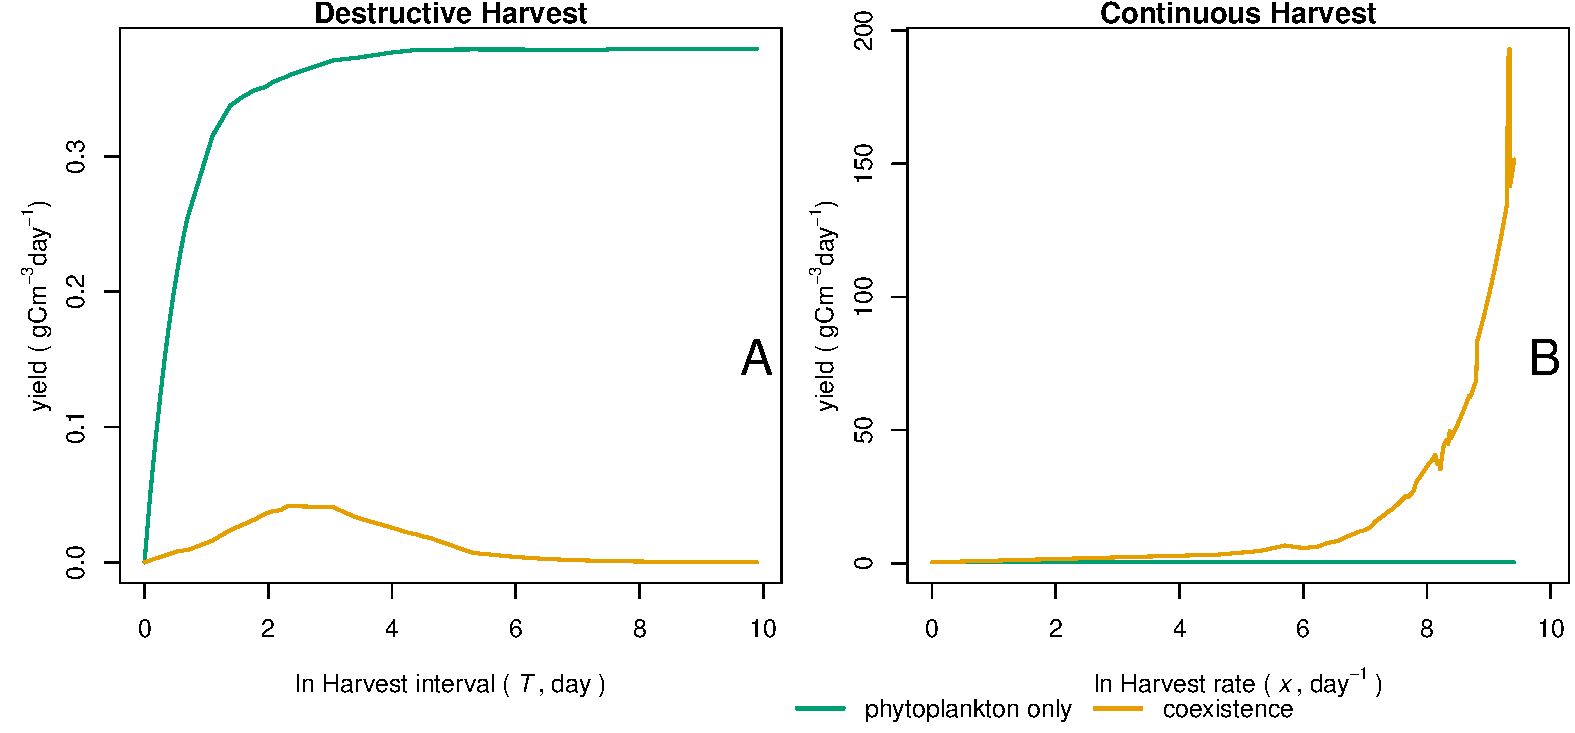
\includegraphics[width=\linewidth]{result/DailyYield.pdf}
    \caption[Median daily yield across systems]{Median daily yield across systems with different unfeasible scenario handling methods.  \textbf{(A)} Yield changes for destructive harvest systems regardless of unfeasible data was treated as invalid (NA) or zeros.  \textbf{(B)} Log yield for continuous harvest systems with unfeasible scenarios treated as invalid data.  \textbf{(C)} Log yield for continuous harvest systems with unfeasible scenarios treated as zero yield.  Note that for \phy-only systems had similar maximum yield (\textbf{A}\&\textbf{C}).  Also note that medians for \PBH\ systems were dominated by feasibility  (\textbf{B}\&\textbf{C}), and feasible scenarios had higher median yield than \phy-only systems \textbf{(B)}.}
    \label{f:ydDaily}
\end{figure}

\begin{figure}[H]
    \centering
    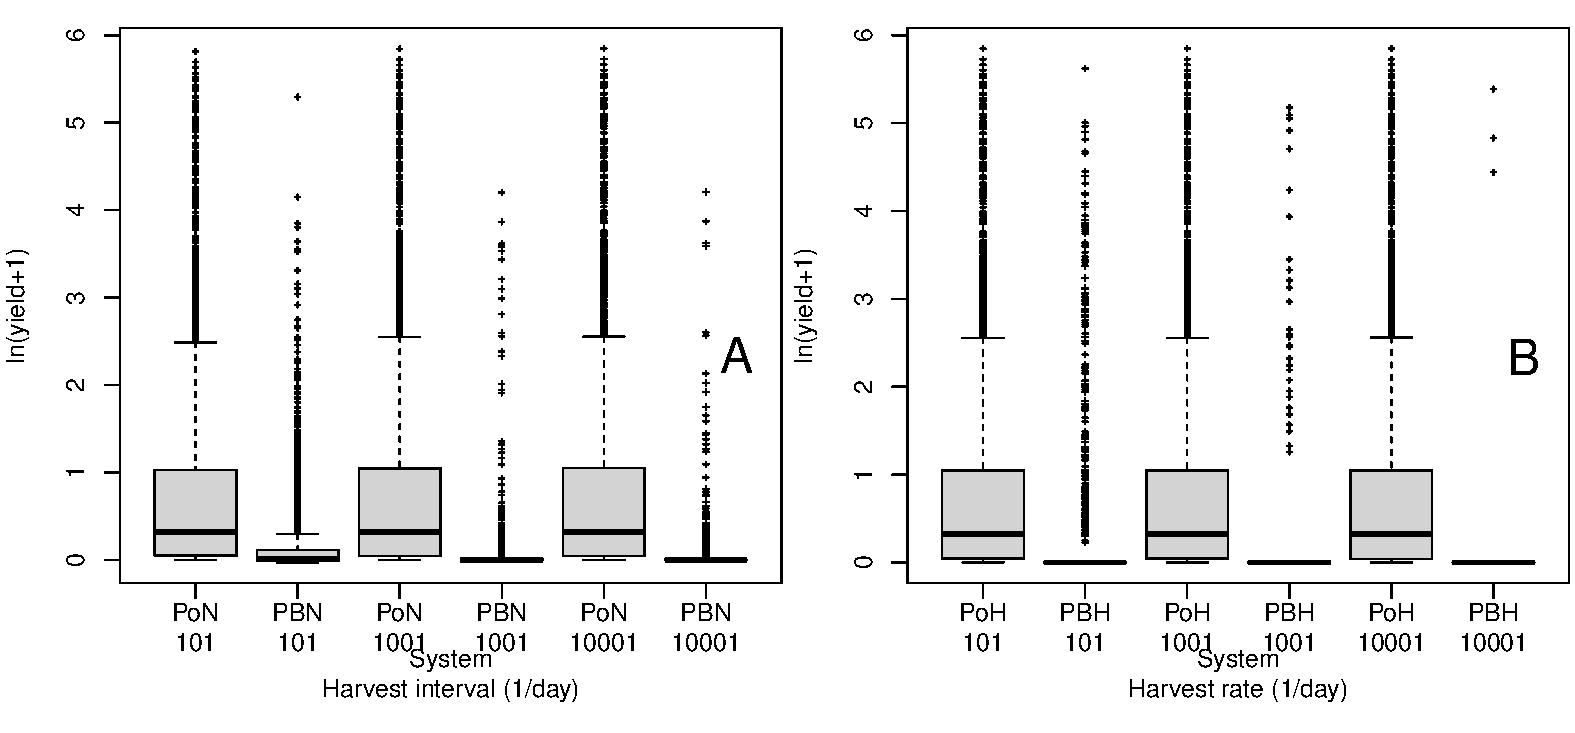
\includegraphics[width=\linewidth]{result/Harvest.pdf}
    \caption[Yield flux distribution by harvest mode]{Log distribution of feasible scenarios on selected harvest interval/rates.  Most boxes had a sample size of 5500, except \PBN\ day 50 (n=5454) and \PBH\ systems in \textbf{(B)} ($x$=100 \dayU, n=184; $x$=1000 \dayU, n=31; $x$=10K \dayU, n=3).  Note that \PoN\ day 0.5 in \textbf{(A)} was the only distribution with median significantly different (pairwise Wilcox p$\ll$0.01) from other \phy-only distributions.  Also note that distributions for \PBH\ systems were dominated by feasibility (\textbf{B}\&\textbf{C}), and feasible scenarios had higher yield distributions than \phy-only systems \textbf{(B)}.}
    \label{f:ydByHarv}
\end{figure}

\begin{figure}[H]
    \centering
    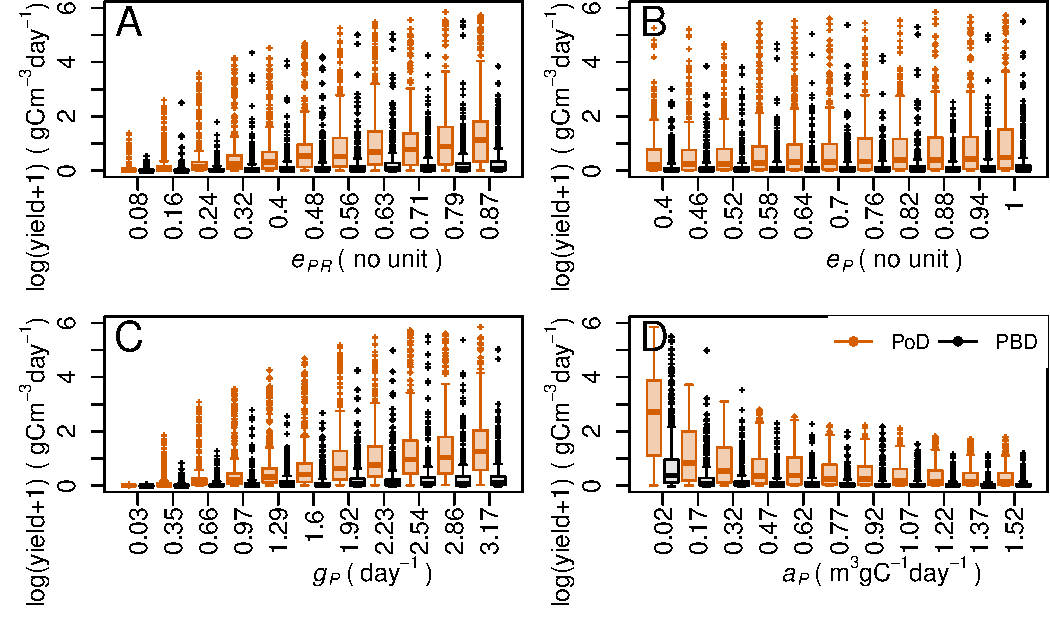
\includegraphics[width=\linewidth]{result/bacEff1.pdf}
    \caption[Log yield flux comparisons between feasible \phy-only and \pbs s]{Log yield flux comparisons between \phy-only and \pbs s on \phy\ parameters.  Note that all parameters had significant influence on both \PoN\ and \PBN\ (Wilcox p$\ll$0.01 between extreme parameter values on both systems).}
    \label{f:bacEffect}
\end{figure}

\begin{figure}[H]
    \centering
    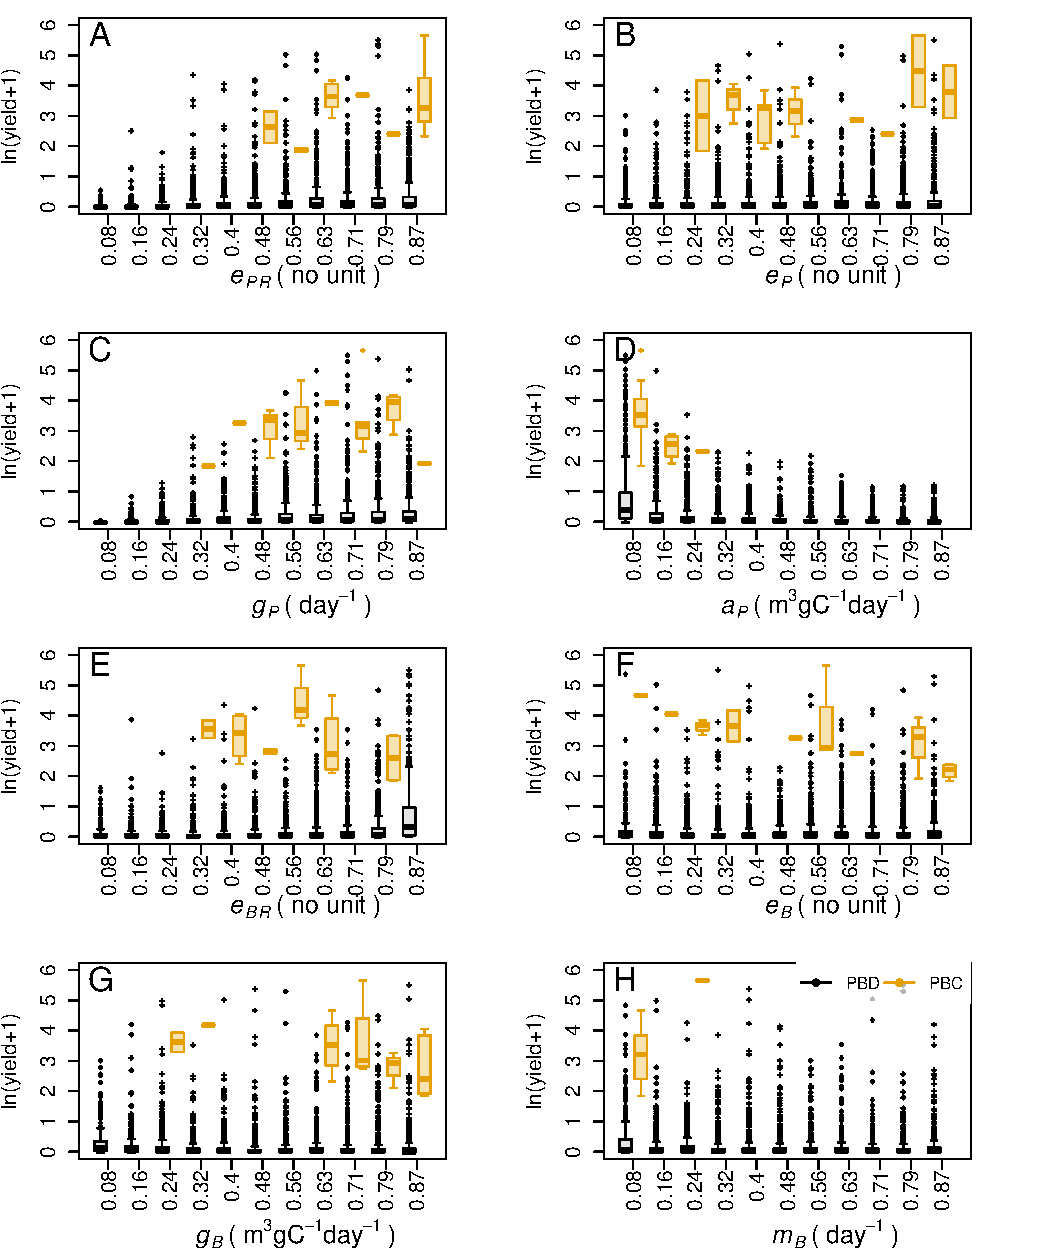
\includegraphics[width=\linewidth]{result/harvB.pdf}
    \caption[Log yield flux comparisons between feasible \pbs s]{Log yield flux comparisons between feasible \pbs s.  Note that \PBH\ feasible distributions were not continuous across parameter ranges with small number of scenarios (n=19) but yielded higher than that of \PBN.  Also note that all parameters had significant influence on both \PBN\ and \PBH\ (Wilcox p$\ll$0.01 between extreme parameter values on both systems).}
    \label{f:harvPB}
\end{figure}

\end{document}